\hypertarget{model_8h}{
\section{model.h File Reference}
\label{model_8h}\index{model.h@{model.h}}
}


This graph shows which files directly or indirectly include this file:\nopagebreak
\begin{figure}[H]
\begin{center}
\leavevmode
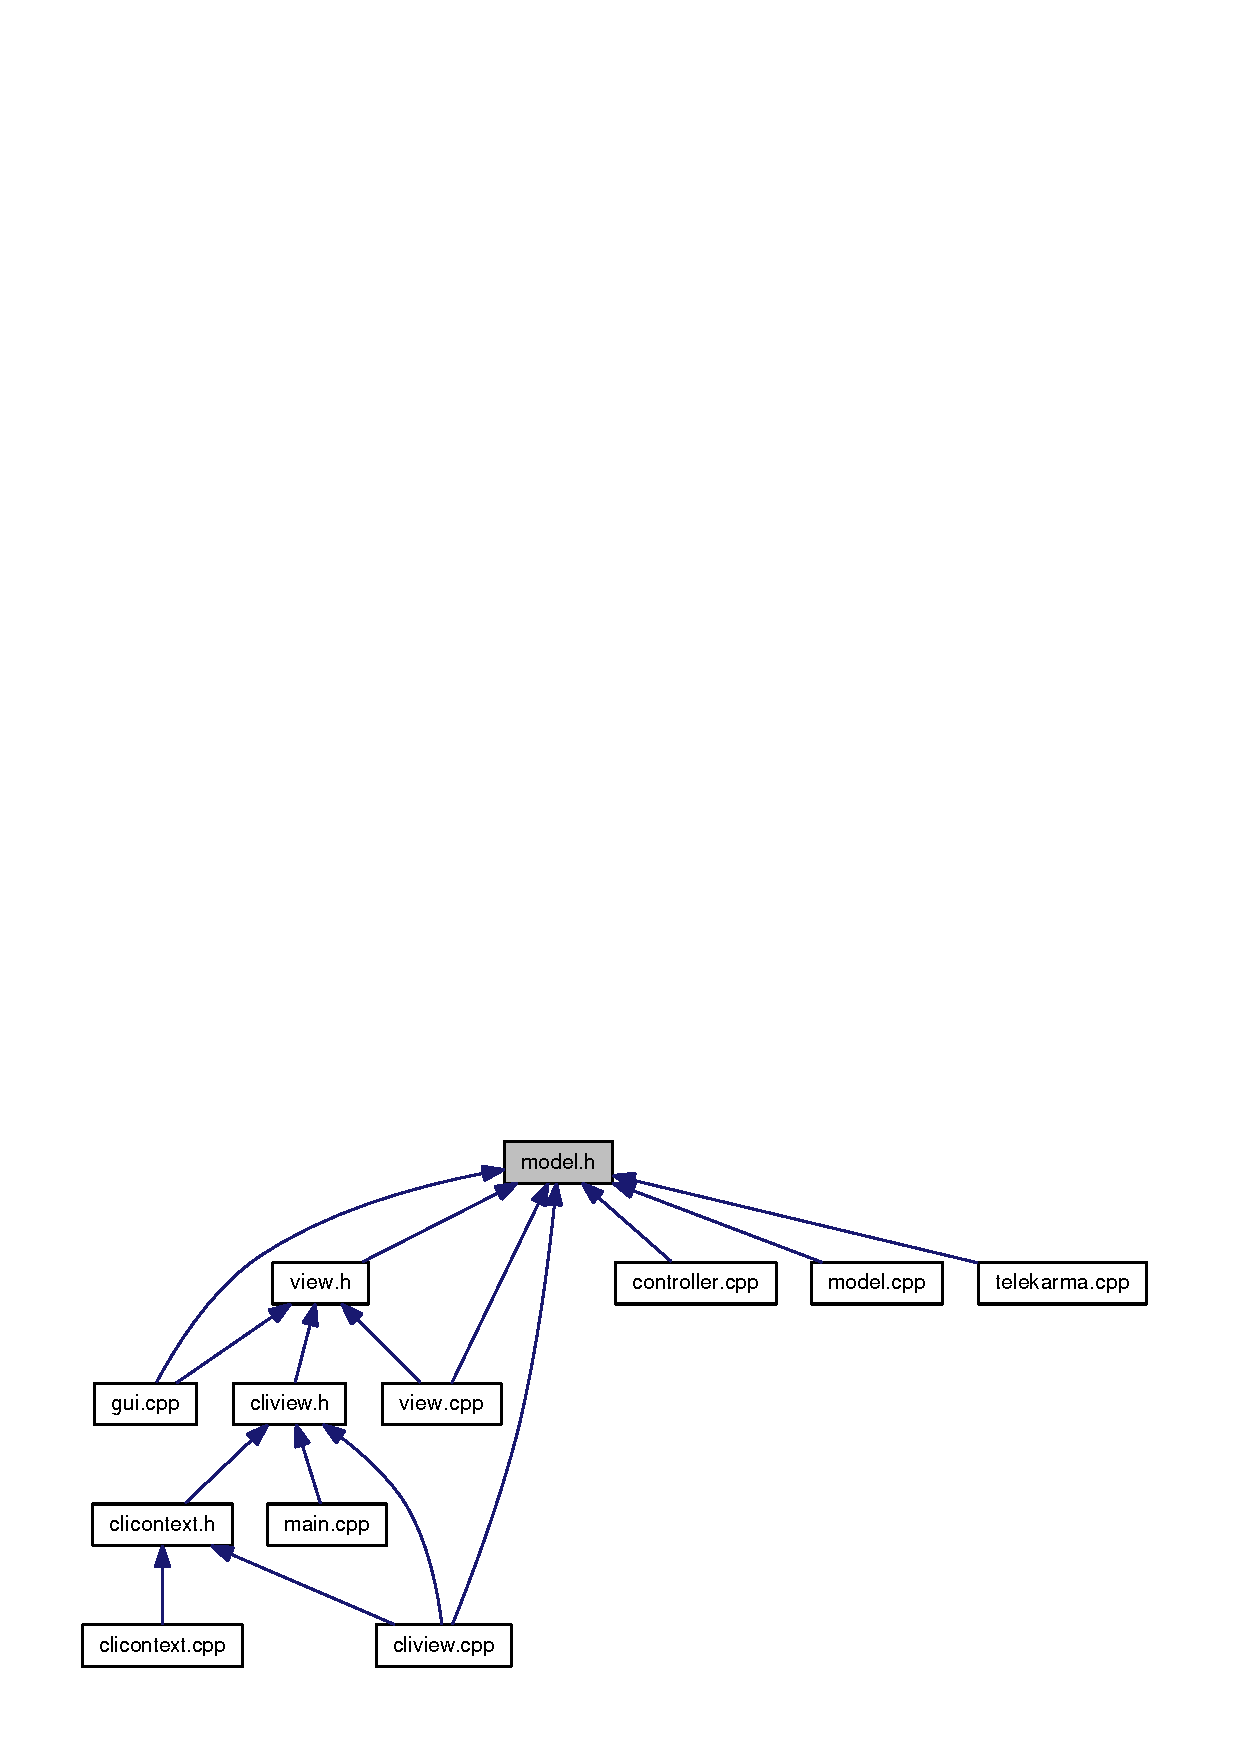
\includegraphics[width=277pt]{model_8h__dep__incl}
\end{center}
\end{figure}
\subsection*{Classes}
\begin{CompactItemize}
\item 
class \hyperlink{classModelListener}{ModelListener}
\item 
class \hyperlink{classModel}{Model}
\end{CompactItemize}
\subsection*{Defines}
\begin{CompactItemize}
\item 
\#define \hyperlink{model_8h_142810068f1b99cd93d3fc9f0e160e02}{QUEUE\_\-SIZE}~50
\begin{CompactList}\small\item\em The default capacity of the action and error message queues. \item\end{CompactList}\end{CompactItemize}


\subsection{Define Documentation}
\hypertarget{model_8h_142810068f1b99cd93d3fc9f0e160e02}{
\index{model.h@{model.h}!QUEUE\_\-SIZE@{QUEUE\_\-SIZE}}
\index{QUEUE\_\-SIZE@{QUEUE\_\-SIZE}!model.h@{model.h}}
\subsubsection[{QUEUE\_\-SIZE}]{\setlength{\rightskip}{0pt plus 5cm}\#define QUEUE\_\-SIZE~50}}
\label{model_8h_142810068f1b99cd93d3fc9f0e160e02}


The default capacity of the action and error message queues. 

